\documentclass{article}
\usepackage[utf8]{inputenc}
\usepackage[T1]{fontenc}
\usepackage{graphicx}
\usepackage{hyperref}
\usepackage{geometry}
\geometry{margin=1in}

\title{THAMANTA}
\date{Encyclopaedia Britannica (1771)}

\begin{document}
\maketitle

\section*{Historical source}
\textbf{Entry ID:} \texttt{entry-thamanta-2171} \\
\textbf{Volume ID:} 144850373 \\
\textbf{Character Count:} 1140

\subsection*{Extracted Text}
THAMANTA, STORKS, a genus of the di-nynia order, belonging to the pantandria claf of plants. Of this genus Limone enumerated nine species; but none of them most particular notice except there-teals, otherwise called \_dance creticus\_. This is an unbeliferous plant growing wild in the Levant and the warranza part of Europe. The leaves are irger-larly dipoled, and formed like thole of fence]. The flower-flake ribs about two feet high, finding out many branches, terminated at the top by compound number, compelled of new zo small ones. There have white flowers with the petals, which are focected by sibling, hairy, channelled fruit, divided into two parts, containing one shloog hairy feed. The feeds have a warm biting tails, with an agreeable aromatic fmell. They are kept in the shape as a medium, are corn-native, and laid to be diverted, but are little tied in practice. The plant may be propagated from feeds, which should be flown on an open bed of light dry ground, the following autumn the plants should be taken up, and planted at about a foot dilness in a bed of light sandy earth, where the roots will continue fo-veral years.



\section*{Source record}
\begin{itemize}
\item \textbf{Dataset:} \texttt{NationalLibraryOfScotland/encyclopaedia\_britannica\_illustrated}
\item \textbf{Dataset Revision:} \texttt{309f765b1ecc83e0a7f7762e44b4a927a7555443}
\item \textbf{Page ID:} \texttt{britannica:309f765b1ecc83e0a7f7762e44b4a927a7555443:train:2171} \\
  \textbf{Filename:} \texttt{page-2171-f8869fa95f19.jpg} \\
  \textbf{Row Index:} 2171 \\
  \textbf{SHA256:} \texttt{f8869fa95f190d0e...}
\end{itemize}

\begin{figure}[h]
\centering
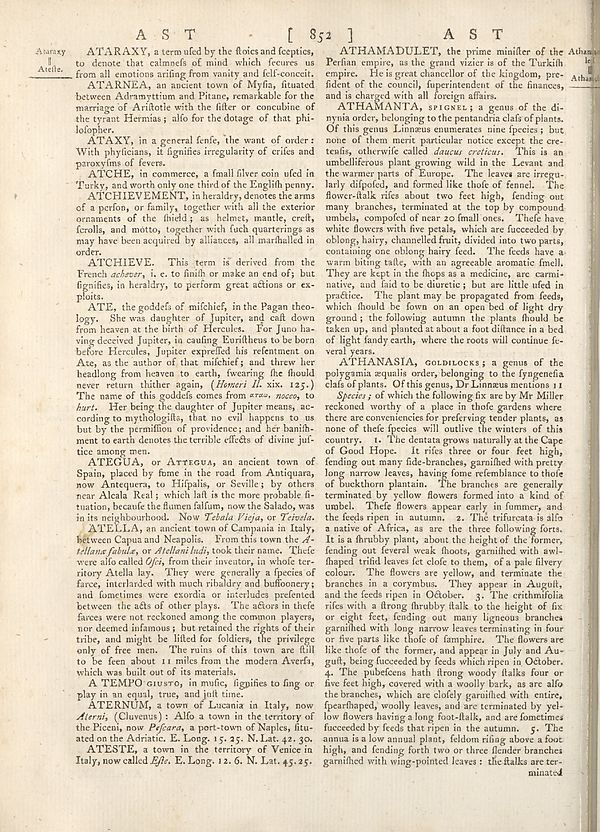
\includegraphics[width=0.85\textwidth]{../scans/page-2171-f8869fa95f19.jpg}
\caption*{Source scan: \texttt{page-2171-f8869fa95f19.jpg}}
\end{figure}

\end{document}
